\Needspace{14\baselineskip}
\section{Results}
\label{sec:results}

\subsection{Study selection}
\label{sec:study-selection}

\autoref{fig:prisma-flow} shows the PRISMA flow diagram.
Searches in Scopus and arXiv, supplemented by citation chasing and one
manual addition, identified 1,194 records.
After removing 83 duplicates, 1,111 records were screened by title and
abstract.
From this screening, 1,060 were excluded and 51 advanced to full-text
reading.

Of the 23 exclusions at the full-text stage, 12 were excluded under EC2
(LLM agents without software engineering evaluation) and 11 under the
IC1/EC1 combination (intra-session retrieval without cross-session
persistence).
Five borderline cases were accepted with documented rationale
(\autoref{sec:selecao}).
The full list of the 23 studies excluded at full-text screening, with
per-criterion exclusion reasons, is available in the replication package
(DOI: 10.5281/zenodo.19463131).
Ultimately, 28 studies were included for data extraction.

% Requer: tikz, calc
\begin{figure}[!htbp]
\centering
\resizebox{\textwidth}{!}{%
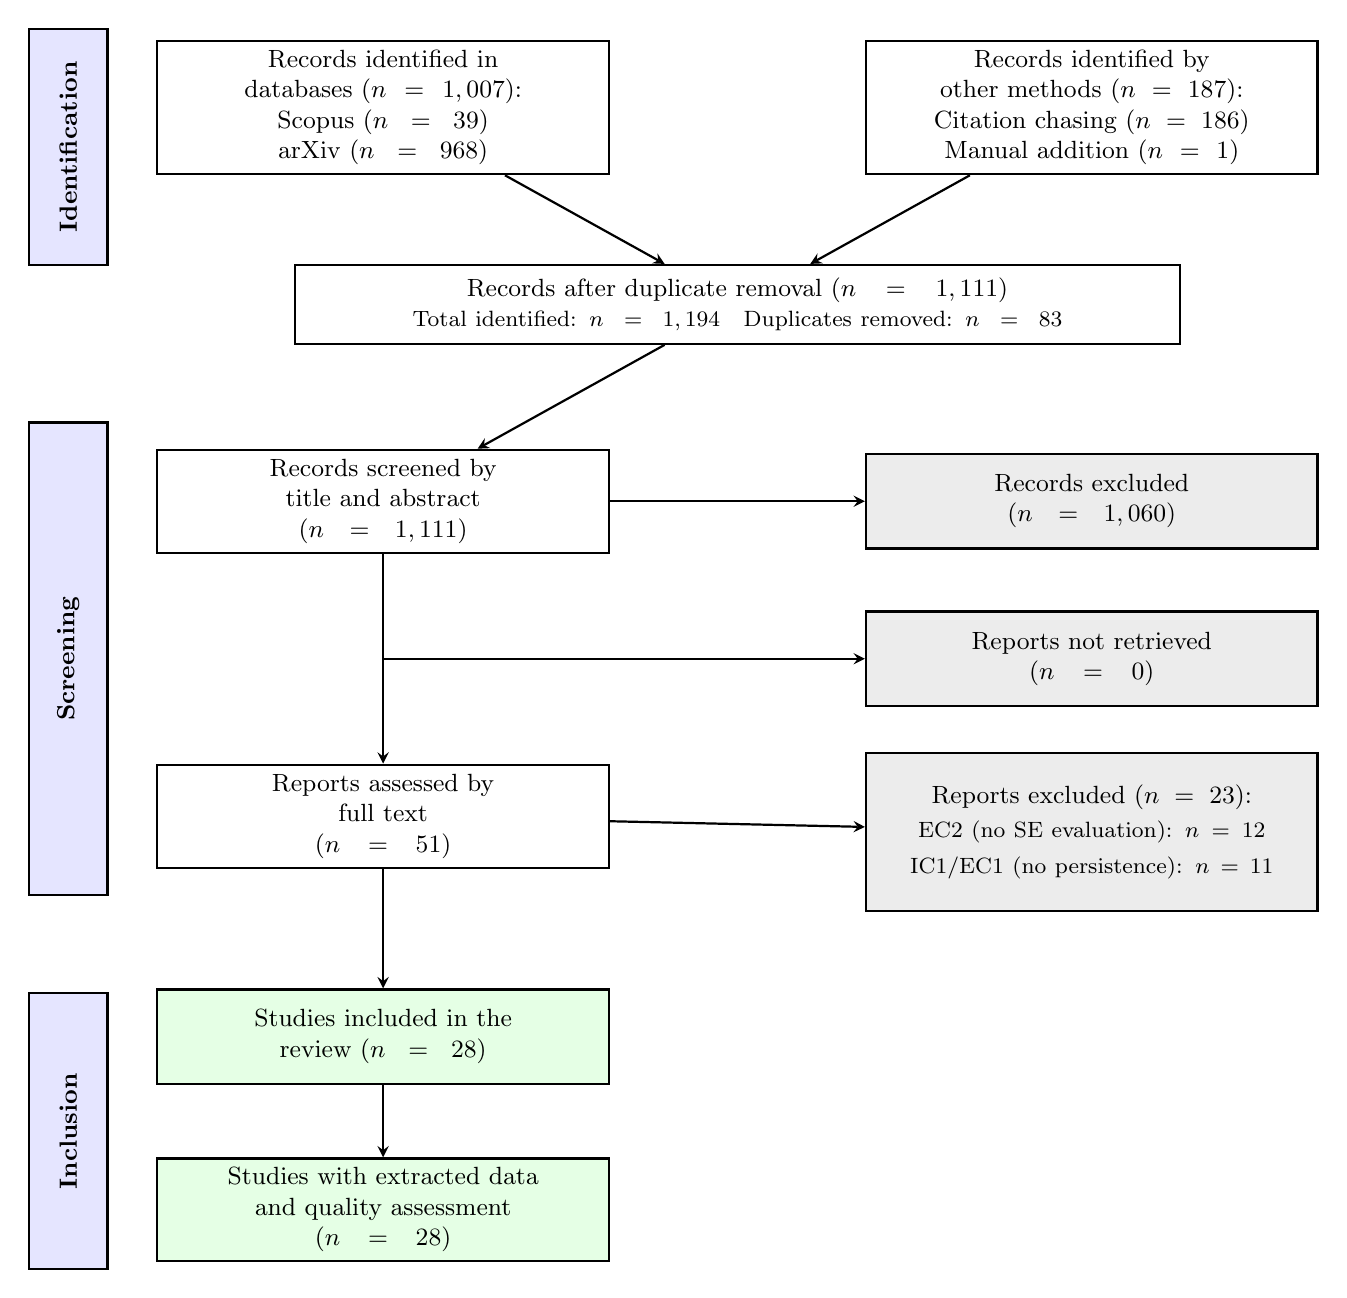
\begin{tikzpicture}[
  box/.style={rectangle, draw=black, thick, text width=5.5cm,
    minimum height=1.2cm, align=center, font=\small},
  boxwide/.style={rectangle, draw=black, thick, text width=11.0cm,
    minimum height=1.0cm, align=center, font=\small},
  boxgray/.style={rectangle, draw=black, thick, fill=gray!15,
    text width=5.5cm, minimum height=1.2cm, align=center, font=\small},
  phaselabel/.style={rectangle, draw=black, thick, fill=blue!10,
    minimum height=1.0cm, align=center,
    font=\small\bfseries, rotate=90, inner sep=3pt},
  arrow/.style={->, thick, >=stealth},
]
\node[phaselabel, minimum width=3.0cm] (l1) at (-2, -0.5)
  {Identification};
\node[phaselabel, minimum width=6.0cm] (l2) at (-2, -7.0)
  {Screening};
\node[phaselabel, minimum width=3.5cm] (l3) at (-2, -13.0)
  {Inclusion};

\node[box] (db) at (2, 0)
  {Records identified in\\databases ($n = 1,007$):\\
   Scopus ($n = 39$)\\arXiv ($n = 968$)};

\node[box] (other) at (11, 0)
  {Records identified by\\other methods ($n = 187$):\\
   Citation chasing ($n = 186$)\\
   Manual addition ($n = 1$)};

\node[boxwide] (dedup) at (6.5, -2.5)
  {Records after duplicate removal ($n = 1,111$)\\
   {\footnotesize Total identified: $n = 1,194$\quad
    Duplicates removed: $n = 83$}};

\draw[arrow] (db) -- (dedup);
\draw[arrow] (other) -- (dedup);

\node[box] (ta) at (2, -5.0)
  {Records screened by\\title and abstract\\($n = 1,111$)};

\node[boxgray] (ta_excl) at (11, -5.0)
  {Records excluded\\($n = 1,060$)};

\draw[arrow] (dedup) -- (ta);
\draw[arrow] (ta) -- (ta_excl);

\node[boxgray] (nr) at (11, -7.0)
  {Reports not retrieved\\($n = 0$)};

\node[box] (ft) at (2, -9.0)
  {Reports assessed by\\full text\\($n = 51$)};

\node[boxgray, minimum height=2.0cm] (ft_excl) at (11, -9.2)
  {Reports excluded ($n = 23$):\\[3pt]
   {\footnotesize
   EC2 (no SE evaluation): $n = 12$\\[2pt]
   IC1/EC1 (no persistence): $n = 11$}};

\draw[arrow] (ta) -- (ft);
\draw[arrow] (2, -7.0) -- (nr.west);
\draw[arrow] (ft) -- (ft_excl);

\node[box, fill=green!10] (incl) at (2, -11.8)
  {Studies included in the\\review ($n = 28$)};

\draw[arrow] (ft) -- (incl);

\node[box, fill=green!10] (qual) at (2, -14.0)
  {Studies with extracted data\\and quality assessment\\($n = 28$)};

\draw[arrow] (incl) -- (qual);

\end{tikzpicture}%
}
\caption{PRISMA 2020 flow diagram for this systematic review.
Adapted from \citet{page2021prisma}.}
\label{fig:prisma-flow}
\end{figure}


\FloatBarrier
\subsection{Characteristics of the included studies}
\label{sec:characteristics}

\autoref{tab:characteristics} summarises the 28 included studies.
All were published between 2024 and 2026; no 2023 study met the
eligibility criteria.
Preprints account for 82\% of the corpus (23 of 28), with two
conference
publications~\citep{wang2026improving,zhang2025darwingodel} and three
workshop
publications~\citep{deshpande2025memtrack,shen2025talm,lindenbauer2025ctimrover}.

Of the 28 included studies, four do not propose a persistence
architecture and are retained as contextual sources
(\autoref{sec:selecao}):
the \citet{du2026memory} analytical survey,
the \citet{deshpande2025memtrack} and \citet{joshi2025swebenchcl}
benchmark proposals, and the \citet{srivastava2025memorygraft} security
evaluation.
The remaining 24 studies are architecture studies relevant to
persistence:
23 propose cross-session persistence architectures, and
Live-SWE-Agent is retained as a task-local executable-memory boundary
case.
They are analysed in the taxonomy;
where the underlying paper reports the relevant data, they also
contribute to the performance (\autoref{sec:sq3}), cost
(\autoref{sec:sq4}), and complexity (\autoref{sec:sq5}) syntheses.
OpenDev~\citep{bui2026opendev}, for example, is included in the SQ1
taxonomy but does not clear the quantitative evaluation floor and is
therefore excluded from SQ3/SQ4/SQ5;
Live-SWE-Agent~\citep{xia2025livesweagent} contributes to the taxonomy
but not as cross-session evidence because its executable tools are
reused within a task and discarded across tasks
(\autoref{sec:selecao}).

Of the 24 architecture studies, 17 share an open repository and three
offer partial access.
The most recurring agent frameworks are custom implementations, followed
by SWE-Agent and OpenHands.
The LLMs used include GPT-4o, Claude 3.5/4/4.5 Sonnet, DeepSeek-V3,
and Gemini 2.5/3 Pro.

\small
\setlength{\tabcolsep}{7pt}
\begin{longtable}{@{}
  >{\raggedright\arraybackslash}p{3.4cm}
  >{\centering\arraybackslash}p{0.7cm}
  >{\raggedright\arraybackslash}p{1.4cm}
  >{\raggedright\arraybackslash}p{1.8cm}
  >{\raggedright\arraybackslash}p{3.8cm}
  S[table-format=1.1]
@{}}
  \caption{Characteristics of the 28 included studies.
    \emph{Role / family}: architecture family for the 24 architecture
    studies and role (survey, benchmark, security) for the 4 contextual
    studies.
    Score: quality score (0--6 scale, per
    \autoref{sec:quality-results}).}
  \label{tab:characteristics} \\
  \toprule
  Study & Year & Venue & Type & Role / family & {Score} \\
  \midrule
  \endfirsthead
  \toprule
  Study & Year & Venue & Type & Role / family & {Score} \\
  \midrule
  \endhead
  \bottomrule
  \endfoot
  Bui (OpenDev) & 2026 & arXiv & preprint & text notes & 2.0 \\
  Chen (SWE-Exp) & 2025 & arXiv & preprint & experience bank & 6.0 \\
  Deng (MemCoder) & 2026 & arXiv & preprint & experience bank & 4.5 \\
  Deshpande (MemTrack) & 2025 & NeurIPS-W & workshop & benchmark & 4.5 \\
  Dong (KernelBlaster) & 2026 & arXiv & preprint & hierarchical/state KB & 4.5 \\
  Du (survey) & 2026 & arXiv & preprint & survey & 2.5 \\
  Guo (EET) & 2026 & arXiv & preprint & experience bank & 5.5 \\
  Hosain (Xolver) & 2025 & arXiv & preprint & hybrid & 5.5 \\
  Joshi (SWE-Bench-CL) & 2025 & arXiv & preprint & benchmark & 5.0 \\
  Li (GBT) & 2026 & arXiv & preprint & executable substrate & 5.5 \\
  Lindenbauer (CTIM-Rover) & 2025 & REALM-W & workshop & experience bank & 4.0 \\
  Nadafian (KAPSO) & 2026 & arXiv & preprint & hybrid & 5.5 \\
  Qian (IER) & 2024 & arXiv & preprint & experience bank & 4.0 \\
  Shen (TALM) & 2025 & AGENT-W & workshop & experience bank & 4.5 \\
  Shen (Structurally) & 2026 & arXiv & preprint & experience bank & 5.0 \\
  Srivastava (MemoryGraft) & 2025 & arXiv & preprint & security & 4.0 \\
  Su (Learn-by-Interact) & 2025 & arXiv & preprint & experience bank & 5.0 \\
  Tablan (Spark) & 2025 & arXiv & preprint & experience bank & 5.0 \\
  Vasilopoulos (Codified) & 2026 & arXiv & preprint & hybrid & 5.0 \\
  Wang (RepoMem) & 2026 & ICLR & conference & repository-history memory & 5.0 \\
  Wang (CodeMEM) & 2026 & arXiv & preprint & AST-guided & 5.0 \\
  Wang (MemGovern) & 2026 & arXiv & preprint & experience bank & 5.5 \\
  Wong (CCA) & 2025 & arXiv & preprint & hybrid & 5.5 \\
  Wu (GCC) & 2025 & arXiv & preprint & Git-style version-control memory & 5.5 \\
  Xia (Live-SWE-Agent) & 2025 & arXiv & preprint & executable substrate (boundary) & 5.5 \\
  Zhang (AccelOpt) & 2025 & arXiv & preprint & experience bank & 5.5 \\
  Zhang (Darwin-Gödel) & 2025 & ICLR & conference & executable substrate & 5.0 \\
  Zhou (ToM-SWE) & 2025 & arXiv & preprint & hybrid & 5.5 \\
\end{longtable}

\autoref{fig:field-map} offers a complementary chronological view of
the corpus, laying out the 28 studies by publication year and
architectural family, with markers for the seven seed papers and for
the three systems whose persistence substrate is executable.

\input{figures/fig-field-map}

\FloatBarrier
\subsection{Quality assessment}
\label{sec:quality-results}

Quality scores range from 2.0 to 6.0, with a median of 5.0.
Twenty-six of the 28 studies (93\%) scored at or above 4.0.
The two studies scoring below
3.0~\citep{bui2026opendev,du2026memory} contribute only qualitative
descriptions; their exclusion in sensitivity analysis S2 does not
alter any quantitative finding.

\FloatBarrier
\subsection{Taxonomy of persistence architectures (SQ1)}
\label{sec:sq1}

\autoref{tab:architectures} shows the distribution of the 24
architecture studies by architecture type.
Eleven studies (46\%) distil resolution trajectories into reusable
entries, making experience banks the most frequent type
(e.g.,~\citep{chen2025sweexp,deng2026memcoder,guo2026eet,shen2026structurally,su2025learnbyinteract}).
Hybrid architectures account for five studies (21\%), typically
combining episodic with semantic
memory~\citep{hosain2025xolver,nadafian2026kapso,wong2025confucius}.
Two implementations use version-control or repository-history memory:
\citet{wang2026improving} mine commit history into episodic and
semantic stores, while \citet{wu2025gcc} exposes a Git-style
version-control memory interface.
Categories such as AST-guided~\citep{wang2026codemem} and
hierarchical/state knowledge base~\citep{dong2026kernelblaster} have
one study each.

\begin{table}[htbp]
  \centering
  \caption{Distribution of the 24 architecture studies by architecture
    type.
    The executable-substrate row includes one task-local boundary case,
    Live-SWE-Agent, whose executable tools are reused within a task but
    discarded across tasks.}
  \label{tab:architectures}
  \begin{tabular}{l r r}
    \toprule
    Architecture type & $N$ & \% \\
    \midrule
    Experience bank       & 11 & 46 \\
    Hybrid                &  5 & 21 \\
    Executable substrate  &  3 & 13 \\
    Repository-history / version-control memory &  2 &  8 \\
    AST-guided            &  1 &  4 \\
    Hierarchical/state KB &  1 &  4 \\
    Text notes            &  1 &  4 \\
    \midrule
    \textbf{Total}      & \textbf{24} & \\
    \bottomrule
  \end{tabular}
\end{table}

The three-dimensional classification proposed by
\citet{du2026memory} enables a more granular analysis.
On temporal scope, 14 studies (58\%) adopt a hybrid scope combining
short- and long-term memory; five (21\%) adopt a procedural scope and
four (17\%) an episodic scope.
Only \citet{wang2026memgovern} uses a purely semantic scope.
The most frequent representational substrate is text-in-context (9
studies, 38\%), followed by structured (7, 29\%) and hybrid (5, 21\%).
Three
studies~\citep{li2026traversalaspolicy,xia2025livesweagent,zhang2025darwingodel}
use executable substrates, where memory takes the form of behaviour
trees, scripts, or entire agents, in contrast with the dominant pattern
of passive data for retrieval.
On control policy, 13 studies (54\%) delegate memory read/write
decisions to the LLM itself, nine (38\%) use fixed heuristics, and two
(8\%) adopt learned policies.

Hybrid retrieval, combining BM25, embeddings, and heuristics, is the
dominant method (11 studies, 46\%).
Full-context memory loading is used only when volume is
compact~\citep{xia2025livesweagent,zhang2025accelopt}.
The predominant granularity is task (16 studies, 67\%), aligned with
benchmark structure in which each issue corresponds to a task.
Cross-agent sharing remains underexplored.
\citet{chen2025sweexp} is the only architecture study that evaluates
memory sharing under a controlled Pass@1 setting, and even there it is
limited to experience reuse within the same framework.
\citet{tablan2025smarter} proposes Spark as a collective shared-memory
layer across coding agents but evaluates a single learning epoch with
synthetic experience and LLM-as-judge metrics, supporting the existence
of shared-memory infrastructure rather than controlled evidence of its
effectiveness.
\autoref{fig:taxonomy} visualises the distribution of studies in the
temporal scope $\times$ substrate space, with colour indicating the
dominant control policy.

\begin{figure}[!htbp]
  \centering
  \resizebox{\textwidth}{!}{\input{figures/fig-taxonomy}}
  \caption{Distribution of the 24 architecture studies in the space of
    temporal scope (rows) $\times$ representational substrate
    (columns).
    Coloured bubbles mark cells that contain at least one study;
    bubble size is proportional to the number of studies in the
    cell, and colour indicates the cell's majority control policy
    (LLM-controlled, heuristic, or no majority when tied).
    Small grey dots mark cells with zero studies and are included
    as grid reference points, not as data.
    The largest cluster is experience-like architectures with a
    hybrid temporal scope, while substrates such as AST-guided,
    hierarchical/state knowledge bases and repository-history or
    version-control memory remain at isolated adoption.}
  \label{fig:taxonomy}
\end{figure}

\FloatBarrier
\subsection{Evaluation methods and benchmarks (SQ2)}
\label{sec:sq2}

Of the 28 included studies, 23 rely on benchmark-only evaluation;
three use non-standard, non-benchmark evaluation:
\citet{bui2026opendev} and \citet{vasilopoulos2026codified} provide
architecture or practitioner case evidence, while
\citet{srivastava2025memorygraft} provide a custom retrieval-level
security evaluation (110 experience seeds, 12 handcrafted queries);
one combines benchmark and case-study evaluation~\citep{zhou2025tomswe};
and one~\citep{du2026memory} is an analytical survey without evaluation
of its own.
The 24 studies with benchmark evaluation (23 benchmark-only plus one
mixed) comprise 22 architecture studies and two contextual benchmark
proposals (MemTrack and SWE-Bench-CL).
ToM-SWE~\citep{zhou2025tomswe} is coded as a hybrid architecture study
whose evaluation combines benchmark results with an observational
user-study component.
\autoref{tab:benchmarks} lists every benchmark used for evaluation
across the 24 studies and the number of studies that adopt each one.
SWE-bench Verified is the most frequent benchmark, used by 13 of the
24 studies with benchmark evaluation (54\%), supplying a partial
comparability anchor across systems even though model, scaffold,
instance subset, and run settings still differ.
Evaluation outside SWE-bench Verified is highly fragmented: only
WebArena and SWE-bench Pro appear in more than one study, with two
studies each, while the remaining 32 benchmarks each appear in a
single study.
This fragmentation spans SWE-bench variants (Lite, Pro, Multilingual,
live, CL, Ambiguous, Stateful), code-generation benchmarks
(HumanEval, BigCodeBench, ClassEval, LiveCodeBench v5, CoderEval,
CodeIF-Bench, DS-1000, SRDD), domain-specific benchmarks
(KernelBench, NKIBench, PyTorch-Bench, Polyglot, MLE-Bench,
ALE-Bench), reasoning and math benchmarks (GSM8K, Math-500, AIME
2024, AIME 2025, GPQA), tool-use and web benchmarks (OSWorld,
Spider2-V, BrowseComp-Plus), safety benchmarks (AgentSafetyBench,
AgentHarm, Agent Security Bench), and the MemTrack benchmark
proposal, limiting direct cross-study comparison.

\begin{table}[htbp]
  \centering
  \caption{Benchmarks and usage frequency across the 24 studies with
    benchmark evaluation, grouped by category.
    \emph{N} counts how many of those studies evaluate on each
    benchmark;
    a single study may evaluate on more than one benchmark (so counts
    do not sum to 24).}
  \label{tab:benchmarks}
  \small
  \setlength{\tabcolsep}{7pt}
  \begin{tabular}{@{} l r @{\hspace{2em}} l r @{}}
    \toprule
    Benchmark & $N$ & Benchmark & $N$ \\
    \midrule
    \multicolumn{4}{@{}l}{\emph{SWE-bench family}} \\
    \quad SWE-bench Verified     & 13 & \quad SWE-bench-live      & 1 \\
    \quad SWE-bench Pro          &  2 & \quad SWE-Bench-CL        & 1 \\
    \quad SWE-bench Lite         &  1 & \quad Ambiguous SWE-bench & 1 \\
    \quad SWE-bench Multilingual &  1 & \quad Stateful SWE        & 1 \\
    \addlinespace
    \multicolumn{4}{@{}l}{\emph{Code generation}} \\
    \quad HumanEval        & 1 & \quad CoderEval    & 1 \\
    \quad BigCodeBench     & 1 & \quad CodeIF-Bench & 1 \\
    \quad ClassEval        & 1 & \quad DS-1000      & 1 \\
    \quad LiveCodeBench v5 & 1 & \quad SRDD         & 1 \\
    \addlinespace
    \multicolumn{4}{@{}l}{\emph{Domain-specific}} \\
    \quad KernelBench   & 1 & \quad Polyglot  & 1 \\
    \quad NKIBench      & 1 & \quad MLE-Bench & 1 \\
    \quad PyTorch-Bench & 1 & \quad ALE-Bench & 1 \\
    \addlinespace
    \multicolumn{4}{@{}l}{\emph{Reasoning and math}} \\
    \quad GSM8K     & 1 & \quad AIME 2025 & 1 \\
    \quad Math-500  & 1 & \quad GPQA      & 1 \\
    \quad AIME 2024 & 1 &                 &   \\
    \addlinespace
    \multicolumn{4}{@{}l}{\emph{Tool-use and web}} \\
    \quad WebArena & 2 & \quad Spider2-V       & 1 \\
    \quad OSWorld  & 1 & \quad BrowseComp-Plus & 1 \\
    \addlinespace
    \multicolumn{4}{@{}l}{\emph{Safety}} \\
    \quad AgentSafetyBench & 1 & \quad Agent Security Bench (ASB) & 1 \\
    \quad AgentHarm        & 1 &                                  &   \\
    \addlinespace
    \multicolumn{4}{@{}l}{\emph{Memory / continual learning}} \\
    \quad MemTrack & 1 &  &  \\
    \bottomrule
  \end{tabular}
\end{table}

Pass@1 (or Resolve Rate) is the dominant metric, adopted by 18 of the
24 studies with benchmark evaluation.
Continual-learning metrics, such as forgetting and backward transfer,
were proposed by \citet{joshi2025swebenchcl} but have not yet been
adopted by other studies.

Direct comparability across systems remains limited.
Although 13 studies use SWE-bench Verified, experimental conditions
differ: at least eight distinct LLMs serve as the backbone, instance
subsets range from CTIM-Rover's 45-instance test
subset~\citep{lindenbauer2025ctimrover} to DGM's 200-task
subset~\citep{zhang2025darwingodel} and the full 500-instance
benchmark, and parameters such as temperature and timeout are rarely
reported.
No study in the corpus compares three or more independent persistence
architectures under the same benchmark, model backbone, scaffold,
compute budget, and cost-accounting protocol.

\FloatBarrier
\subsection{Performance results (SQ3)}
\label{sec:sq3}

Nineteen architecture studies present controlled comparisons against a
no-persistence or non-memory baseline.
Eighteen report positive aggregate results in their main controlled
comparison; one, CTIM-Rover~\citep{lindenbauer2025ctimrover}, reports
negative results across all CTIM configurations.
\autoref{tab:performance} lists the 18 comparisons with gains measurable
in percentage points (pp), drawn from 17 unique studies because
\citet{su2025learnbyinteract} contributes separate OSWorld and
SWE-bench Verified rows;
Dong~\citep{dong2026kernelblaster} and
Tablan~\citep{tablan2025smarter} are discussed separately because they
use non-comparable metrics (speedup and qualitative score).
Across the 18 percentage-point comparisons the median gain is
+7.8~pp;
within the SWE-bench Verified subset ($n=12$, including CTIM-Rover) the
median is +6.5~pp.
Magnitudes range from $-2.0$~pp~\citep{lindenbauer2025ctimrover} to
+39.0~pp~\citep{li2026traversalaspolicy}.
Gains that combine persistence with changes in search, tooling,
orchestration, or evaluation budget (for example,
KAPSO~\citep{nadafian2026kapso}, DGM~\citep{zhang2025darwingodel}, and
GCC~\citep{wu2025gcc}) should be read as full-system gains relative to
each study's own baseline rather than as isolated estimates of the
memory component.

\begin{table}[htbp]
  \centering
  \caption{Percentage-point comparisons against the no-persistence
    baseline, sorted by gain.
    Rows are comparisons, not studies:
    Su~(Learn-by-Interact) contributes two benchmark rows, and gains
    without within-study memory ablations are full-system gains.}
  \label{tab:performance}
  \begin{tabular}{l l r r r}
    \toprule
    Study & Benchmark & Base (\%) & Mem. (\%) & Gain \\
    \midrule
    Li (GBT) & SWE-b. V. & 34.6 & 73.6 & +39.0~pp \\
    Zhang (DGM) & SWE-b. V. & 20.0 & 50.0 & +30.0~pp \\
    Nadafian (KAPSO) & MLE-Bench & 35.1 & 50.7 & +15.6~pp \\
    Wang (CodeMEM) & CodeIF-B. & $\sim$73 & 85.2 & +12.2~pp \\
    Zhou (ToM-SWE) & Ambig. SWE & 51.9 & 63.4 & +11.5~pp \\
    Su (LbI) & OSWorld & 12.4 & 22.5 & +10.1~pp \\
    Deng (MemCoder) & SWE-b. V. & 68.4 & 77.8 & +9.4~pp \\
    Wang (MemGovern) & SWE-b. V. & 23.2 & 32.6 & +9.4~pp \\
    Su (LbI) & SWE-b. V. & 51.2 & 60.0 & +8.8~pp \\
    Shen (Struct.) & SWE-b. V. & 53.5 & 60.3 & +6.8~pp \\
    Wu (GCC) & SWE-b. V. & 74.0 & 80.2 & +6.2~pp \\
    Wang (RepoMem) & SWE-b. V. & 37.0 & 40.4 & +3.4~pp \\
    Shen (TALM) & BigCodeB. & 50.1 & 53.3 & +3.2~pp \\
    Xia (Live-SWE) & SWE-b. V. & 74.2 & 77.4 & +3.2~pp \\
    Wong (CCA) & SWE-b. Pro & $\sim$56 & 59.0 & +3.0~pp \\
    Guo (EET) & SWE-b. V. & $\sim$32 & $\sim$35 & +2.7~pp \\
    Chen (SWE-Exp) & SWE-b. V. & 70.8 & 73.0 & +2.2~pp \\
    Lindenbauer (CTIM-Rover) & SWE-b. V. subset & 42.0 & 40.0 & $-2.0$~pp \\
    \bottomrule
  \end{tabular}
\end{table}

The two largest SWE-bench Verified gains come from the weakest
baselines: \citet{li2026traversalaspolicy} starts at 34.6\% and gains
+39.0~pp, and \citet{zhang2025darwingodel} starts at 20.0\% and gains
+30.0~pp;
\citet{su2025learnbyinteract} on OSWorld (not SWE-bench Verified) also
starts low (12.4\%) and gains +10.1~pp.
Low baselines do not, however, uniformly imply gains above 10~pp:
\citet{wang2026memgovern} starts at 23.2\% on SWE-bench Verified and
reports a gain of 9.4~pp.
On SWE-bench Verified, studies with baselines above 65\% report gains
between +2.2 and +9.4~pp (Chen 70.8\%~$\to$~+2.2; Xia 74.2\%~$\to$~+3.2;
Wu 74.0\%~$\to$~+6.2; Deng 68.4\%~$\to$~+9.4).
The data are consistent with diminishing returns as the system
approaches the benchmark ceiling, but this pattern is descriptive and
not formally tested.

Cross-LLM effects are configuration-dependent.
\citet{shen2026structurally} reports an average gain of +4.7~pp across
four distinct LLMs, and \citet{wang2026memgovern} reports +4.65~pp on
average across seven LLMs for its governed full system.
Within-study ablations, however, show inversions:
Live-SWE-Agent~\citep{xia2025livesweagent} degrades GPT-5-Nano from
44.0\% to 14.0\% and GPT-5-Mini from 60.0\% to 58.0\% on its ablation
subset,
TALM~\citep{shen2025talm} reports that memory hurts HumanEval with both
GPT-4o-mini (90.59\%~$\to$~89.13\%) and GPT-4o (94.48\%~$\to$~92.55\%),
and MemGovern's raw-experience standard-RAG variant decreases
Qwen3-Coder from 48.0\% to 46.8\%.
The evidence supports model- and configuration-dependent persistence
effects rather than a uniform cross-LLM benefit.
\autoref{fig:gains} visualises per-study gains, with colour indicating
architecture type.

\begin{figure}[!htbp]
  \centering
  \input{figures/fig-gains}
  \caption{Gain in percentage points ($\Delta$~pp) over the
    no-persistence baseline, for the 18 comparable
    percentage-point comparisons reported by 17 unique studies.
    Each bar corresponds to a comparison, with colour indicating
    the memory-architecture type;
    Su~(Learn-by-Interact) contributes two benchmark rows.
    Across the 18 comparisons the median gain is 7.8~pp; within
    the SWE-bench Verified subset ($n = 12$, including
    CTIM-Rover) the median is 6.5~pp.
    The two largest gains (above 10~pp) come from systems starting
    from baselines below 35\%, but within that baseline range some
    studies remain below 10~pp (e.g., MemGovern: baseline
    23.2\%, gain 9.4~pp).
    On SWE-bench Verified, studies with baselines above 65\%
    report gains between 2.2 and 9.4~pp; the data suggest
    diminishing returns without formally testing it.
    CTIM-Rover~\citep{lindenbauer2025ctimrover} appears as the only
    controlled negative case ($-2.0$~pp relative to the
    AutoCodeRover baseline in its best configuration).
    Dong (KernelBlaster) and Tablan (Spark) are omitted because
    they use non-comparable metrics (speedup and qualitative
    score, respectively).}
  \label{fig:gains}
\end{figure}

Five architecture studies are excluded from the percentage-point SQ3
synthesis because they lack a comparable no-persistence coding-agent
baseline, use non-standard proxy metrics, or compare against baselines
that do not isolate persistence:
\citet{bui2026opendev}, \citet{vasilopoulos2026codified},
\citet{qian2024iterative}, \citet{hosain2025xolver}, and
\citet{zhang2025accelopt}.

\FloatBarrier
\subsection{Cost and efficiency (SQ4)}
\label{sec:sq4}

Cost reporting is heterogeneous.
Among the 24 architecture studies, seven report monetary cost per task
with enough supporting detail (tokens, model, configuration) for
study-level cost interpretation;
nine report partial data (cost or tokens, but not both);
and eight report no cost data (33\%).
Only a subset of the cost-reporting studies provide a within-study
memory-vs-no-memory cost delta;
the remainder report component ablations, full-system comparisons, or
non-comparable partial cost figures rather than against an ablated
memory baseline.
Adding the four contextual studies raises the count to 12 of the 28
included studies (43\%) that do not contribute cost data, including
the Du survey, for which the cost field is not applicable.
Cost underreporting is therefore visible under both denominators:
the architecture corpus (33\%) and the full included corpus (43\%).

\autoref{tab:cost-evidence} distinguishes the cost evidence types
considered during SQ4 coding.
The distinction matters because only the first type estimates the
incremental operating cost of persistence under a fixed system and
backbone.

\begin{table}[htbp]
  \centering
  \caption{Cost evidence types considered in SQ4.}
  \label{tab:cost-evidence}
  \small
  \begin{tabularx}{\textwidth}{@{} l X X @{}}
    \toprule
    Evidence type & Meaning & Examples in this corpus \\
    \midrule
    Memory delta &
      Same system and backbone, with memory or persistence ablated &
      EET, SWE-Exp, MemGovern \\
    Component ablation &
      One memory component removed or isolated inside the same system &
      CodeMEM CtxMem/SessAST, KernelBlaster KB, TALM memory module \\
    Full-system comparison &
      Scaffold, model, or orchestration changes together with memory &
      TALM vs.\ MapCoder, GCC vs.\ other agents, AccelOpt vs.\
      Claude~Sonnet~4 \\
    Single configuration &
      Cost reported without a comparable memory baseline &
      None retained after strict SQ4 coding \\
    \bottomrule
  \end{tabularx}
\end{table}

\autoref{tab:cost} reports monetary cost per task in the studies that
publish it, with the evidence type interpreted according to
\autoref{tab:cost-evidence}.
AccelOpt~\citep{zhang2025accelopt} is included because it provides a
detailed monetary breakdown, but its headline 26-fold cost reduction
compares an open-source backbone with experience queue against a
Claude~Sonnet~4 baseline, not a within-study memory-versus-no-memory
contrast.
This result is therefore not counted as a persistence-cost effect, and
AccelOpt is omitted from \autoref{fig:cost} for the same reason.
Variation is wide: from \$0.01 per
task~\citep{guo2026eet} to \$7.27~\citep{wang2026memgovern},
reflecting differences in the LLM backbone, the benchmark, and the
underlying architecture.

\begin{table}[htbp]
  \centering
  \caption{Monetary cost per task in studies that report monetary data,
    grouped by LLM configuration where the study presents several.
    The seven studies with monetary cost and supporting detail (Chen,
    Guo, MemGovern, Wu, Xia, Zhang AccelOpt, and Zhou) have at least
    one row; Wang RepoMem is included despite partial detail because
    it reports monetary cost per task.
    Not every row is a within-study memory-vs-no-memory contrast; see
    \autoref{fig:cost} for the subset with a within-study cost delta.}
  \label{tab:cost}
  \small
  \setlength{\tabcolsep}{4pt}
  \begin{tabular}{l r l l l}
    \toprule
    Study & Cost/task & LLM & Benchmark & Evidence \\
    \midrule
    Guo (EET) & \$0.01 & GPT-5-mini & SWE-b. V. & Memory delta \\
    Zhou (ToM-SWE) & \$0.02 & GPT-5-nano & Stateful SWE & Memory delta \\
    Xia (Live-SWE) & \$0.05--0.73 & various & SWE-b. V./Pro & Memory delta \\
    Wang (MemGov., Qwen) & \$0.07 & Qwen3-30B & SWE-b. V. & Memory delta \\
    Chen (SWE-Exp) & \$0.13 & DeepSeek-V3 & SWE-b. V. & Memory delta \\
    Wu (GCC) & \$0.57--1.21 & various & SWE-b. Lite & Full-system \\
    Wang (RepoMem) & \$0.58--0.89 & NR & SWE-b. V. & Memory delta \\
    Zhang (AccelOpt) & \$6.87--15.95 & open-source & NKIBench & Full-system \\
    Wang (MemGov., Claude) & \$7.27 & Claude 4 S. & SWE-b. V. & Memory delta \\
    \midrule
    \multicolumn{5}{l}{\footnotesize NR: not reported in the original paper.} \\
    \bottomrule
  \end{tabular}
\end{table}

Among studies with within-study memory-vs-baseline cost comparisons,
the relationship between memory and cost follows two distinct patterns.
Systems that use memory to replace redundant context reduce costs:
\citet{guo2026eet} achieves $-31.8$\% in total cost,
\citet{li2026traversalaspolicy} cuts tokens by 39\%, and
\citet{dong2026kernelblaster} reports 2.4$\times$ fewer tokens than a
minimal no-KB agent.
\citet{shen2025talm} reports roughly half the tokens of MapCoder on
ClassEval, but that is a full-system comparison;
the memory module itself adds only marginal token overhead and is not
counted as a within-study persistence-cost reduction.
For CodeMEM, the plotted token reduction refers to the Code Context
Memory (CtxMem) component;
removing the session-memory SessAST component reduces tokens further
but also reduces performance.
By contrast, systems that add context via retrieval increase costs
marginally:
\citet{chen2025sweexp} reports $+7.5$\% in tokens and
\citet{wang2026memgovern} $+4.8$\% with Claude 4 Sonnet.
In these cases, the performance gains are accompanied by added cost;
the corpus does not report a formal relationship between the
magnitudes of gain and cost.
\autoref{fig:cost} illustrates this duality.

\begin{figure}[!htbp]
  \centering
  \resizebox{\textwidth}{!}{% Requer: tikz (já carregado em main.tex)
% Source: extraction/extracted-data.tsv (study, cost_impact, cost_mechanism)
\begin{tikzpicture}[
  font=\small,
  system box/.style={
    draw=#1!70, fill=#1!10, rounded corners=3pt,
    minimum width=3.8cm, minimum height=0.7cm,
    align=center, font=\footnotesize,
  },
  system box/.default=archBanco,
  group label/.style={
    font=\small\bfseries, align=center,
  },
  arrow down/.style={-Stealth, thick, black!60},
]
\node[group label, text=posGain] at (-3.5, 0)
  {Replacement\\[-2pt]{\footnotesize (reduces cost)}};
\node[group label, text=negLoss] at (3.5, 0)
  {Addition\\[-2pt]{\footnotesize (raises cost)}};

\draw[dashed, black!30, thick] (0, 0.5) -- (0, -6.5);
\node[system box=posGain] at (-3.5, -1.0)
  {EET: $-31.8$\% cost};
\node[system box=posGain] at (-3.5, -2.0)
  {GBT: $-39$\% tokens};
\node[system box=posGain] at (-3.5, -3.0)
  {TALM: $\sim$$-50$\% tokens};
\node[system box=posGain] at (-3.5, -4.0)
  {KernelBlaster: $2.4\times$ fewer tokens};
\node[system box=posGain] at (-3.5, -5.0)
  {CodeMEM CtxMem: $-30$k tokens/round};
\node[system box=posGain] at (-3.5, -6.0)
  {CCA: $-11$k tokens/task};
\node[system box=negLoss] at (3.5, -2.0)
  {SWE-Exp: $+7.5$\% tokens};
\node[system box=negLoss] at (3.5, -3.0)
  {MemGovern: $+4.8$\% cost};
\node[system box=negLoss] at (3.5, -4.0)
  {Live-SWE: $+4$--$21$\%};
\node[system box=negLoss] at (3.5, -5.0)
  {RepoMem: higher cost on hard tasks};
\node[font=\scriptsize, text=black!60, align=center,
  text width=3.5cm] at (-3.5, -7.2)
  {Memory replaces redundant\\context or avoids\\rework};
\node[font=\scriptsize, text=black!60, align=center,
  text width=3.5cm] at (3.5, -6.2)
  {Memory adds context\\via retrieval; accuracy\\gains come with\\higher cost};

\end{tikzpicture}
}
  \caption{Schematic of the two opposite patterns of memory impact on
    operating cost among studies that provide a within-study cost or
    token delta against a no-persistence or ablation comparator.
    On the left, systems that substitute condensed memory for
    redundant context (e.g., EET, Traversal-as-Policy, KernelBlaster)
    report cost reductions.
    On the right, systems that add context via retrieval (e.g.,
    SWE-Exp, MemGovern with Claude~4~Sonnet) report cost increases.
    Entries are qualitative and are not directly comparable across
    studies.}
  \label{fig:cost}
  \par\smallskip
  \footnotesize\emph{Note.}
  Entries use the cost variable reported by each original study and are
  directional, not directly comparable across studies.
  TALM and AccelOpt are excluded from the plotted persistence-cost
  effects because their headline reductions are full-system or
  backbone-changing comparisons.
  \normalsize
\end{figure}

Among studies with within-study persistence-cost comparisons,
\citet{guo2026eet} provides the clearest cost-saving result:
$-31.8$\% in total cost with at most a $-0.2$~pp loss in resolve rate
in the authors' setting, by identifying early-termination opportunities
in 11.3\% of issues.
Separately, \citet{zhang2025accelopt} reports a 26-fold cost reduction
relative to Claude Sonnet~4 with comparable performance in its
domain;
this result compares an open-source backbone with experience queue
against a different model backbone and is therefore not counted as a
persistence-cost effect.
No study constructs a cross-architecture Pareto frontier under the same
benchmark, model backbone, scaffold, compute budget, and
cost-accounting protocol.
ToM-SWE reports a configuration-level cost-performance frontier, and
other papers provide cost-performance curves or single-system cost
breakdowns, but none compares multiple persistence architectures under
the same benchmark, model backbone, scaffold, compute budget, and
cost-accounting protocol.
Cross-study dominance on both axes cannot be established directly:
benchmarks, base models, and cost-accounting conventions differ among
the studies that report cost data.

\FloatBarrier
\subsection{Complexity versus effectiveness (SQ5)}
\label{sec:sq5}

Nine of the 28 included studies (32\%) report adverse outcomes
associated with knowledge persistence.
\autoref{tab:degradation} groups these cases by mechanism category and
indicates which are direct regressions, overhead, security, or
evaluation-artefact findings.

\begin{table}[htbp]
  \centering
  \caption{Adverse or cautionary findings related to persistence and
    its evaluation, grouped by mechanism category.
    Four cases include a direct performance drop or benchmark-level
    regression; the remainder capture overhead, security, or evaluation
    artefacts.}
  \label{tab:degradation}
  \small
  \setlength{\tabcolsep}{5pt}
  \begin{tabularx}{\textwidth}{@{} >{\raggedright\arraybackslash}p{2.0cm} >{\raggedright\arraybackslash}p{2.4cm} >{\raggedright\arraybackslash}p{2.9cm} >{\raggedright\arraybackslash}X @{}}
    \toprule
    Study & Category & Mechanism & Scenario \\
    \midrule
    Lindenbauer & Performance drop & retrieval noise &
      Noisy CTIM injection diverts exploration;
      best CTIM configuration is $-2$~pp, weakest CTIM-only variants
      fall to $-11$~pp \\
    Chen & Performance drop & retrieval noise &
      retrieving $k > 1$ experiences degrades performance
      (42.0\% to 39.0\%) \\
    Deshpande & Benchmark caution & backend redundancy, follow-up decay &
      Mem0 and Zep do not improve aggregate correctness, increase
      tool-call redundancy to $\sim$21\%, and perform worse than no-memory
      on follow-up-question conditions \\
    Xia & Performance drop & model-dependent overhead &
      GPT-5-Nano: 44.0\%~$\to$~14.0\% ($-30$~pp;
      $-68.2$\% relative) under tool creation \\
    \midrule
    Shen (TALM) & Overhead & unnecessary retrieval &
      Retrieval does not pay off on simple tasks;
      memory also reduces HumanEval accuracy with GPT-4o-mini
      (90.59\%~$\to$~89.13\%) and GPT-4o (94.48\%~$\to$~92.55\%) \\
    Vasilopoulos & Overhead & maintenance burden &
      24.2\% knowledge-to-code ratio is diagnostic, not a target;
      reported upkeep averaged 1--2 h/week and stale specs caused
      silent failures \\
    \midrule
    Srivastava & Security & memory poisoning &
      9.1\% poisoned experiences appear in 47.9\% of retrieved records
      under dual-channel retrieval; downstream behavioural severity is
      not measured \\
    \midrule
    Joshi & Evaluation artefact & framework incompatibility &
      Chronological ordering of tasks incompatible with the memory
      mechanism \\
    Zhou & Evaluation artefact & simulator bias &
      User simulator introduces over-compliance \\
    \bottomrule
  \end{tabularx}
\end{table}

Four mechanism categories emerge from the data.
Four studies report direct performance drops or benchmark-level
regressions in their main or coded adverse comparison:
retrieval noise~\citep{lindenbauer2025ctimrover,chen2025sweexp},
backend redundancy with follow-up decay~\citep{deshpande2025memtrack},
and model-dependent overhead~\citep{xia2025livesweagent};
\citet{shen2025talm} also report sub-benchmark drops on HumanEval
when memory is enabled, even though their main BigCodeBench result
(\autoref{tab:performance}) is positive.
Deshpande is retained as benchmark-level cautionary evidence rather
than as an architecture-level SQ3 degradation result.
TALM is coded as an overhead case because its main coded benchmark
comparison is positive, but it also reports memory-enabled HumanEval
drops.
The four direct performance-drop cases should therefore be read as main
or coded adverse comparisons, not as every negative sub-result in the
corpus.
Two report overhead or maintenance burden rather than direct
main-comparison drops~\citep{shen2025talm,vasilopoulos2026codified};
one documents a security vulnerability in open experience stores
(memory poisoning)~\citep{srivastava2025memorygraft};
and two document evaluation artefacts that complicate interpretation
without establishing performance degradation:
evaluation-framework incompatibility with chronological task
ordering~\citep{joshi2025swebenchcl} and user-simulator
bias~\citep{zhou2025tomswe}.

Adding memory layers is not, by itself, evidence of a better agent.
\citet{zhang2025accelopt}, with a simple experience queue, and
\citet{guo2026eet}, with a termination heuristic, obtain substantial
gains in their respective domains without resorting to multi-tier
architectures such as KAPSO~\citep{nadafian2026kapso} and
GCC~\citep{wu2025gcc}.
The factor with the strongest apparent association to gain is the
distance between the baseline and the benchmark's potential ceiling:
simple memory applied to a weak
baseline~\citep{zhang2025darwingodel} produces +30~pp, while
sophisticated memory on a strong
baseline~\citep{chen2025sweexp} yields +2.2~pp.

Retrieval calibration is a major design variable in the studies that
isolate it.
\citet{chen2025sweexp} reports that retrieving more than one experience
degrades the result (42.0\% to 39.0\% with $k = 4$), and
\citet{shen2026structurally} shows that category isolation outperforms
global retrieval by +2.3~pp.
Across the negative cases, the recurring issue is weak governance of
what enters the prompt:
excessive retrieval, unfiltered CTIM items, stale specifications, or
low-quality stored trajectories.

\FloatBarrier
\subsection{Sensitivity analyses and certainty}
\label{sec:sensitivity}

Two sensitivity analyses verified the stability of the findings.
The first (S1) kept only the five studies published in peer-reviewed
venues.
The headline direction of the findings does not invert, but SQ4 becomes
much weaker:
detailed monetary cost evidence is largely removed, and only two
peer-reviewed architecture studies retain partial cost/token relevance
(RepoMem~\citep{wang2026improving} and
TALM~\citep{shen2025talm}).
The second (S2) excluded the two studies scoring below 3.0.
The removal does not alter SQ3 or SQ4 because neither study contributes
to the performance or cost synthesis: Du is a non-architecture
contextual source, and OpenDev is an architecture study that does not
clear the IC2 quantitative floor and is used only for the SQ1
taxonomy.
For SQ1, excluding OpenDev removes the single text-notes substrate
but does not change the dominance of experience banks.

\autoref{tab:certainty} presents the per-finding certainty assessment.
Each row also receives an evidence-type classification:
\textbf{A} for direct data extracted from the TSV or JSON (counts,
percentages, exhaustive checks), \textbf{B} for cross-study patterns
aggregated from multiple studies, and \textbf{C} for mechanism
characterisations or causal inferences whose empirical base is
inherently interpretive.
Certainty refers to confidence in the extracted finding, not to causal
identification of the memory component unless explicitly stated.
After merging the duplicated Gap~1 row, the table reports 18 findings:
12 receive high certainty, five receive moderate certainty, and one
receives low certainty;
in parallel, 12 are classified as type A, four as type B, and two as
type C.
The only low-certainty finding is SQ1-D (executable substrates, based
on only three studies), while SQ5-B (relation between complexity and
gain) receives moderate certainty because it relies on comparison
across studies with different benchmarks.

\FloatBarrier

Preprints dominate the corpus (82\%), which introduces reporting-bias
risk, particularly for SQ4 (cost data, frequently absent in preprints)
and SQ2 (benchmark selection, less standardised in non-peer-reviewed
work).
Sensitivity analysis S1, restricted to the five studies published in
peer-reviewed venues, did not invert any finding, which suggests that
reporting-bias risk is contained for the high-certainty findings.
For findings with moderate or low certainty (\autoref{tab:certainty}),
preprint influence cannot be ruled out.

\FloatBarrier

\begin{table}[htbp]
  \centering
  \caption{Certainty and evidence type per finding.
  Certainty refers to confidence in the extracted finding, not to causal
  identification of the memory component unless explicitly stated.
  Type A: direct data (counts, percentages).
  Type B: aggregated cross-study pattern.
  Type C: mechanism characterisation or causal inference.}
  \label{tab:certainty}
  \small
  \setlength{\tabcolsep}{7pt}
  \begin{tabularx}{\textwidth}{@{} >{\raggedright\arraybackslash}p{5.4cm} >{\centering\arraybackslash}p{0.7cm} >{\centering\arraybackslash}p{1.5cm} >{\raggedright\arraybackslash}X @{}}
    \toprule
    Finding & Type & Certainty & Rationale \\
    \midrule
    SQ1-A: banks dominate (46\%) & A & high & 11 studies, direct count \\
    SQ1-B: hybrid scope (58\%) & A & high & 14 studies \\
    SQ1-C: LLM controls memory (54\%) & A & high & 13 studies, direct
      classification \\
    SQ1-E: hybrid retrieval (46\%) & A & high & 11 studies \\
    SQ1-F: sharing underexplored & A & high &
      22 of 24 report no sharing proposal; Chen is the only study with
      controlled evidence, Tablan proposes infrastructure without
      controlled evaluation \\
    SQ2-A: SWE-bench V. most frequent & A & high & 13 of 24 benchmark-evaluated studies \\
    SQ2-D: no head-to-head comparison & A & high & exhaustive check \\
    SQ3-A: mostly positive controlled evidence, one negative case & B & high &
      18 positive studies, 1 negative (CTIM-Rover) \\
    SQ4-A: cost underreported (8/24 architecture; 12/28 full) & A & high &
      direct count; denominator reported separately for architecture corpus
      and full included corpus \\
    SQ4-D: no cross-architecture Pareto frontier & A & high &
      exhaustive check; ToM-SWE reports a configuration-level frontier
      within one architecture \\
    SQ5-A: 32\% adverse outcomes & A & high & 9 studies with evidence \\
    T-A: field dominated by preprints (82\%) & A & high & direct count \\
    \midrule
    SQ3-B: diminishing returns & B & moderate & observed pattern,
      not formally tested \\
    SQ3-C: cross-LLM effects configuration-dependent & B & moderate &
      2 multi-LLM studies show average gains; ablations and alternative
      configurations show inversions \\
    SQ4-B: two cost patterns & B & moderate &
      cost/token deltas reported with heterogeneous metrics \\
    SQ5-B: complexity $\neq$ gain & C & moderate & cross-study
      inference, heterogeneous benchmarks \\
    SQ5-D: retrieval calibration & C & moderate & 2 direct studies \\
    \midrule
    SQ1-D: executable substrates & A & low & only 3 studies \\
    \bottomrule
  \end{tabularx}
\end{table}
